% !TeX program = ptex2pdf -u -l
\documentclass[11pt,a4paper]{jsarticle}
%
\usepackage{amsmath,amssymb}
\usepackage{bm}
\usepackage[dvipdfmx]{graphicx}
\usepackage{ascmac}
\usepackage{atbegshi}
\usepackage[dvipdfmx]{geometry} % 追加: 余白を一時的に0にするため(dvipdfmx指定)
\usepackage{listings} % ソースコード表示のために追加
\usepackage{float}
\usepackage{tcolorbox}
\newtcbox{\code}[1][]{
  colback=gray!10!white,
  colframe=gray!20!white,
  boxrule=0.5pt,
  left=2pt,right=2pt,top=1pt,bottom=1pt,
  box align=base,
  fontupper=\ttfamily
}
% 簡易コード表示用マクロ(本文中で\textttt{...}を使えるようにする)
\newcommand{\textttt}[1]{\texttt{#1}}
%ここからソースコードの表示に関する設定
\lstset{
  basicstyle={\ttfamily},
  identifierstyle={\small},
  commentstyle={\small\itshape},
  keywordstyle={\small\bfseries},
  ndkeywordstyle={\small},
  stringstyle={\small\ttfamily},
  frame={tb},
  breaklines=true,
  columns=[l]{fullflexible},
  numbers=left,
  xrightmargin=0zw,
  xleftmargin=3zw,
  numberstyle={\scriptsize},
  stepnumber=1,
  numbersep=1zw,
  lineskip=-0.5ex
}
\renewcommand{\lstlistingname}{ソースコード} % キャプションを「ソースコード」に変更
%ここまでソースコードの表示に関する設定
\newcommand{\myPdfAuthor}{平田爽馬/HIRATA,Soma}
\newcommand{\myPdfTitle}{電源回路の基礎実験}
\AtBeginShipoutFirst{\special{pdf:tounicode EUC-UCS2}} % pLaTeXの内部漢字コードがEUCの場合
\AtBeginDvi{\special{pdf:docinfo <<
 /Author   (\myPdfAuthor)
 /Title    (\myPdfTitle)>>}}
%
\setlength{\textwidth}{\fullwidth}
\setlength{\textheight}{40\baselineskip}
\addtolength{\textheight}{\topskip}
\setlength{\voffset}{-0.2in}
\setlength{\topmargin}{0pt}
\setlength{\headheight}{0pt}
\setlength{\headsep}{0pt}
%
\newcommand{\divergence}{\mathrm{div}\,}  %ダイバージェンス
\newcommand{\grad}{\mathrm{grad}\,}  %グラディエント
\newcommand{\rot}{\mathrm{rot}\,}  %ローテーション
%
\title{\myPdfTitle}
\author{5E25番 平田爽馬}
\date{}
\begin{document}
%\maketitle%タイトルを挿入したくない場合は,消す
%
%
\section{目的}
ダイオードを用いた電源回路にといて,交流を直流にする整流回路や整流波形から脈動分を除去する平滑回路の動作を調べる.
また,応用回路として,3端子レギュレータ,チョッパ電源回路についての動作も調べ理解を深める.

\section{原理}
一般に.電源回路はトランスと整流回路,平滑回路から構成される.
以降,整流回路と平滑回路,応用回路について簡単に説明する.

\subsection{電源回路の基礎}
図\ref{fig1}のように直流で動作する電子回路を動作させるためには,交流である商用電源から整流・平滑により直流にする交流-直流変換の電圧源や電池など,不安定な直流電圧を安定化電源により安定した電圧に変換して供給する.\\
本節では,直流-直流変換の電源回路(安定化電源)の種類と特徴を解説し,交流から直流に変換する整流・平滑回路について説明する.

\begin{figure}[H]
\centering
\includegraphics[width=85mm]{./fig/fig1.eps}
\caption{負荷である電子回路への電源構成}
\label{fig1}
\end{figure}

\subsubsection{電源回路の種類と特徴}
不安定な直流電圧から安定した直流電圧に変換する安定化電源は,図\ref{fig2}に示すように方式や回路構成によって分類できる.
\begin{figure}[H]
\centering
\includegraphics[width=85mm]{./fig/fig2.eps}
\caption{電源回路(安定化電源)の分類}
\label{fig2}
\end{figure}

また,電源回路の基本的な構成は図\ref{fig3}のようになり,出力の電圧検出回路の出力と基準電圧回路の出力を制御回路により比較して,出力トランジスタなどのエネルギー変換素子を制御することで$V_o$を一定にする.

\begin{figure}[H]
\centering
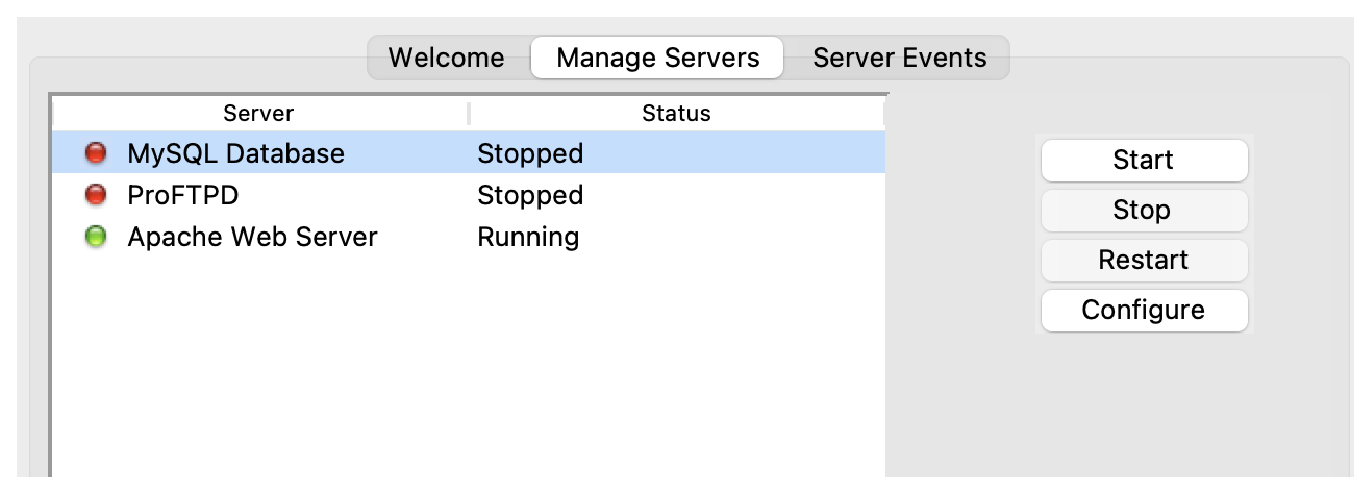
\includegraphics[width=80mm]{./fig/fig3.eps}
\caption{電源回路の基本構成}
\label{fig3}
\end{figure}

\subsubsection*{リニア方式およびスイッチング方式の特徴}
図\ref{fig2}のリニア方式とスイッチング方式についてそれぞれ特徴を述べる.
\paragraph{リニア方式}\quad\\
リニア方式は,制御回路とエネルギー変換素子である出力トランジスタは線形アナログ動作領域のみで動作して一定の出力電源を発生する.回路構成により山とレギュレータとシリーズレギュレータに分けられる.\\
リニア方式の電源には次のような特徴がある.
\begin{itemize}
\item 高い電源電圧から低い出力電圧に変換する降圧型のみである.
\item 出力電流=入力電流となるため,電力損失は入力と出力の電圧差に比例する.
\item 出力トランジスタを線形アナログ動作領域で制御するため出力にノイズが発生しない.
\item 出力トランジスタとトランジスタを中心に構成した制御回路や基準電圧で回路を構成できるため半導体に集積可能である.
\end{itemize}

\paragraph{スイッチング方式}\quad\\
スイッチング方式には,エネルギー変換素子としてインダクタやキャパシタと出力トランジスタを用い,制御回路により入力側電源からの電流を出力トランジスタでオン・オフさせることでインダクタやキャパシタに蓄積するエネルギーを制御して,一定の電圧を出力する.

スイッチング方式は出力トランジスタをオン・オフさせて制御することから非線形回路となる.
そして,エネルギー変換阻止部分の構成により,入力電源電圧に対して低い電圧を出力する降圧型,逆に高い電圧を出力する昇圧型,降圧型と昇圧型の両方を動作する昇降圧型,入力電源い対して逆の極性の電源を出力する斑点型に分けられる.\\
スイッチング方式の電源には次のような特徴がある.
\begin{itemize}
\item 入力電力と出力電力をほぼ等しくすることができて電力損失が少なく高効率である.
\item 出力トランジスタのオン・オフにより出力にノイズが生じる.
\item エネルギー変換素子としてインダクタやキャパシタを使用するので半導体に集積するのは容易ではなく,電源回路構成によって複雑になる.
\end{itemize}

\subsubsection*{電源の性能を評価する項目}
主に,以下の項目で電源の性能を評価する.
\begin{itemize}
\item ラインレギュレーション:静的動作時において入力電圧変動に対して出力電圧変動の度合いを評価する.
\item ロードレギュレーション:静的動作時において負荷電流変動に対して出力電圧変動の度合いを評価する.
\item リップル:静的動作時において出力電圧の変動幅(出力電圧の最大・最小の差)を評価する.
\item 効率:入力電力と出力電力の比率(出力電力/入力電力)を評価する.
\end{itemize}
このほか,出力抵抗,負荷過渡応答回復時間などがある.

\section{実験}
\subsection{実験1:半波整流回路}

\begin{figure}[H]
\centering
\includegraphics[width=75mm]{./fig/fig4.eps}
\caption{半波整流回路の回路図}
\label{fig4}
\end{figure}

\subsubsection*{実験}
\begin{itemize}
  \item 図\ref{fig4}の回路を組み立てる.
  \item 変圧器の二次側の電圧$V_1$と出力$V_o$の波形をオシロスコープにより観測し,記録する.
\end{itemize}

\subsubsection*{結果}

\begin{figure}[H]
\centering
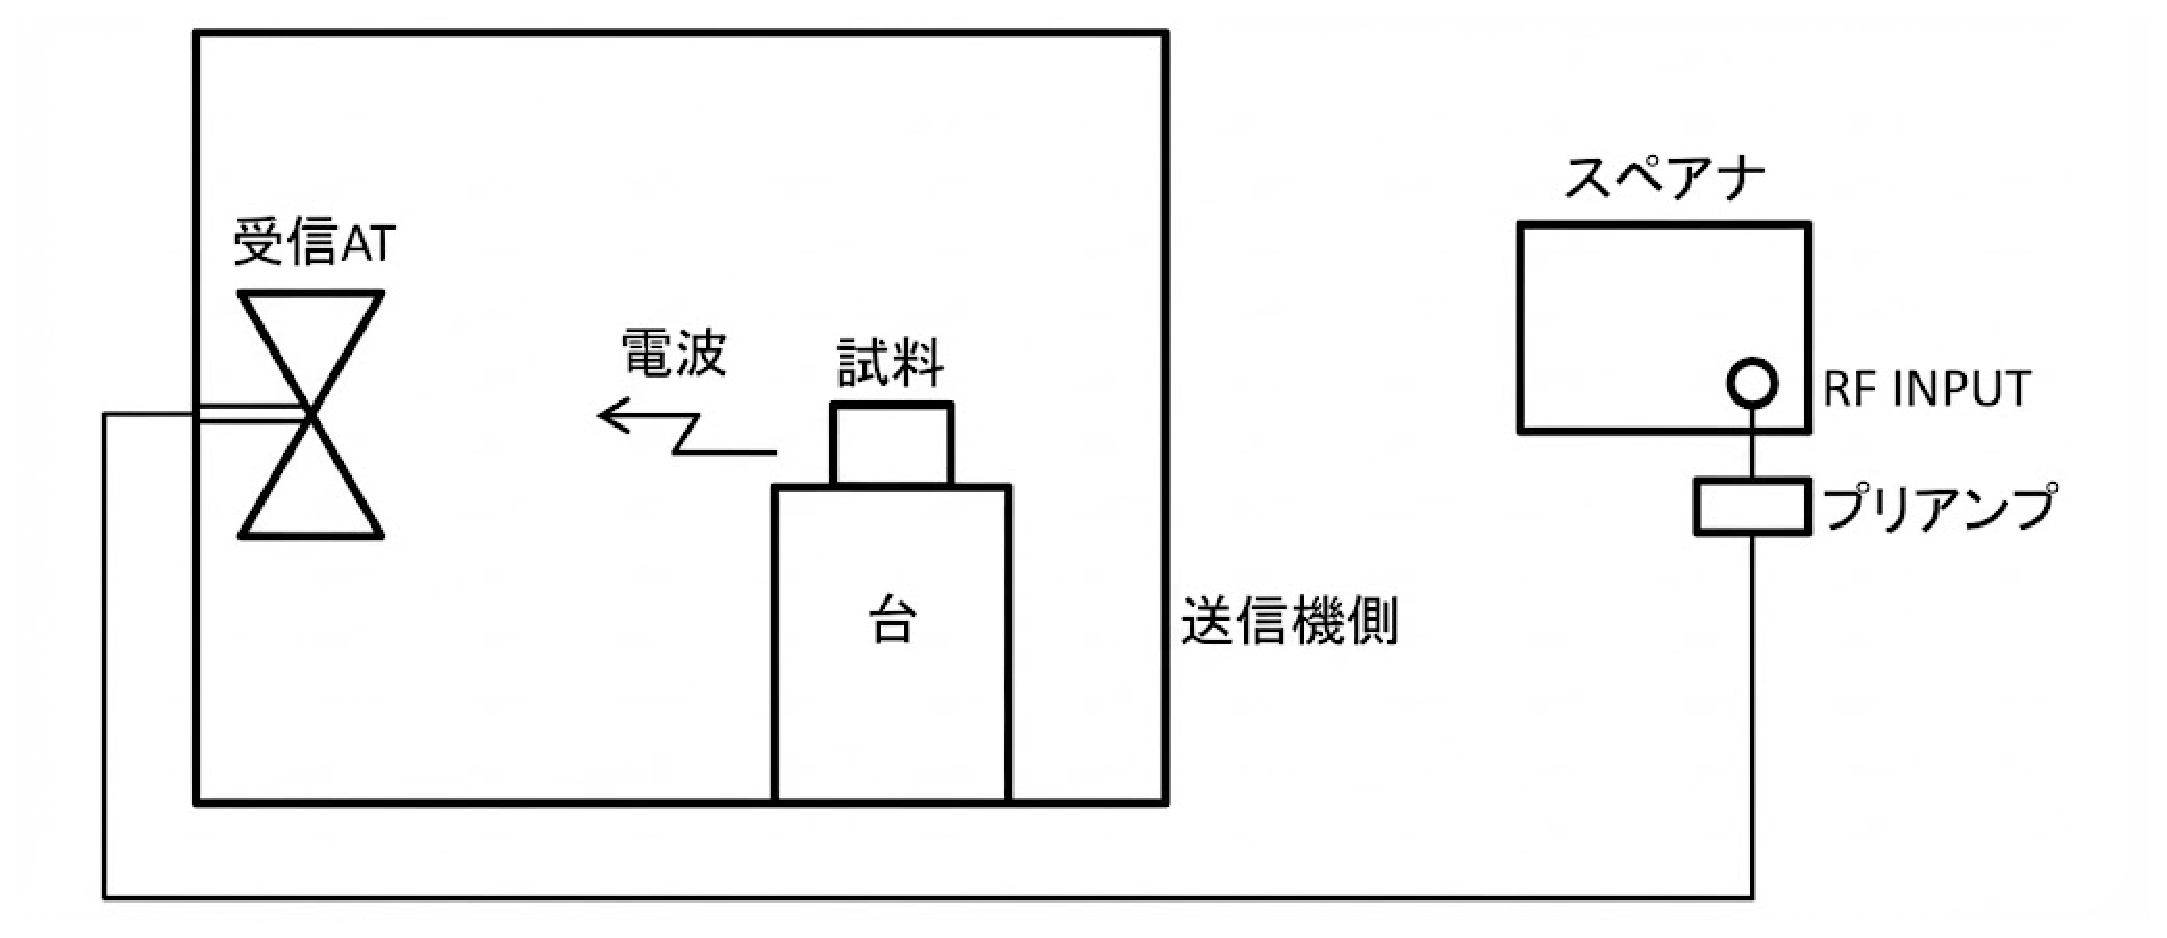
\includegraphics[width=75mm]{./fig/fig5.eps}
\caption{作製した半波整流回路}
\label{fig5}
\end{figure}

図\ref{fig5}に作製した半波整流回路を示す.

\begin{figure}[H]
\centering
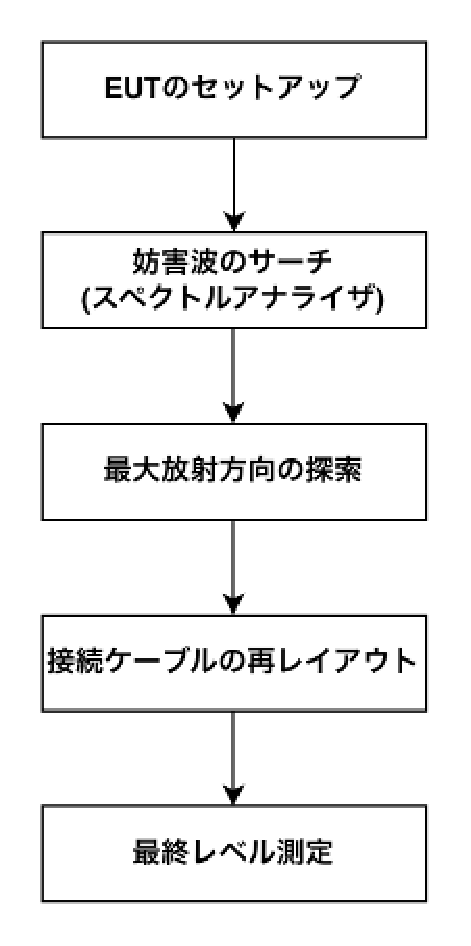
\includegraphics[width=75mm]{./fig/fig6.eps}
\caption{二次側の電圧と出力の波形}
\label{fig6}
\end{figure}

図\ref{fig6}に二次側の電圧$V_1$と出力$V_o$の波形を示す.

\subsubsection*{考察1}
半波整流回路の出力電圧のピーク値を$V_{\rm{max}}$としたときの,出力電圧$V_o$の平均値$\bar{V_o}$を導出する.
\begin{gather}
\bar{V_o}=\frac{1}{2\pi}\int_{0}^{2\pi}V_od\theta \\
\bar{V_o}=\frac{1}{2\pi}\int_{0}^{\pi}V_{\rm{max}}\sin\theta d\theta + \frac{1}{2\pi}\int_{\pi}^{2\pi}0 d\theta\\
\bar{V_o}=\frac{1}{2\pi}(V_{\rm{max}}(-\cos(\pi)+\cos(0))+0) \\
\bar{V_o}=\frac{1}{2\pi}(2V_{\rm{max}}) \\
\bar{V_o}=\frac{V_{\rm{max}}}{\pi}
\end{gather}

\subsection{実験2:全波整流回路}

\begin{figure}[H]
\centering
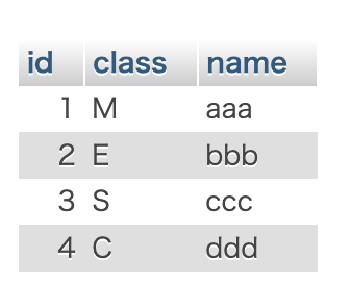
\includegraphics[width=80mm]{./fig/fig7.eps}
\caption{全波整流回路の回路図}
\label{fig7}
\end{figure}

\subsubsection*{実験}
\begin{itemize}
  \item 図\ref{fig7}の回路を組み立てる.$R_L=2[kΩ]$.
  \item 変圧器の二次側の電圧$V_1$と出力$V_o$の波形をオシロスコープにより観測し,記録する.
\end{itemize}

\subsubsection*{結果}

\begin{figure}[H]
\centering
\includegraphics[width=80mm]{./fig/fig8.eps}
\caption{作製した全波整流回路}
\label{fig8}
\end{figure}

図\ref{fig8}に作製した全波整流回路を示す.

\begin{figure}[H]
\centering
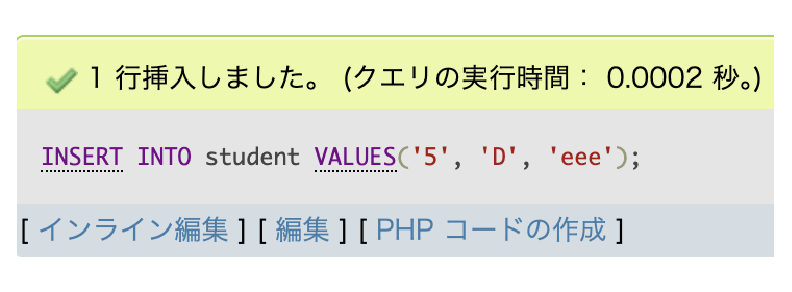
\includegraphics[width=80mm]{./fig/fig9.eps}
\caption{二次側の電圧と出力の波形}
\label{fig9}
\end{figure}

図\ref{fig9}に二次側の電圧$V_1$と出力$V_o$の波形を示す.
\newpage

\subsubsection*{考察2}
全波整流回路の出力電圧のピーク値を$V_{\rm{max}}$としたときの,出力電圧$V_o$の平均値$\bar{V_o}$を導出する.

\begin{gather}
\bar{V_o}=\frac{1}{\pi}\int_{0}^{\pi}V_{\rm{max}}\sin (\theta)d\theta \\
\bar{V_o}=\frac{1}{\pi}(V_{\rm{max}}(-\cos(\pi)+\cos(0))) \\
\bar{V_o}=\frac{1}{\pi}(2V_{\rm{max}}) \\
\bar{V_o}=\frac{2V_{\rm{max}}}{\pi}
\end{gather}

\subsection{実験3:コンデンサによる平滑回路を持つ全波整流回路}

\begin{figure}[H]
\centering
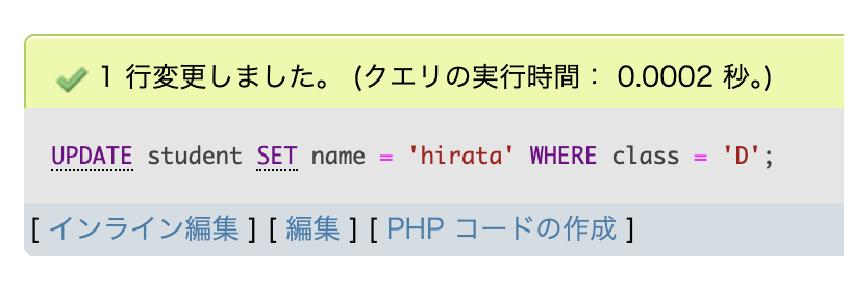
\includegraphics[width=80mm]{./fig/fig10.eps}
\caption{コンデンサによる平滑回路を持つ全波整流回路の回路図}
\label{fig10}
\end{figure}

\subsubsection*{実験}
\begin{itemize}
  \item 図\ref{fig10}の回路を組み立てる.$R_L=2[kΩ]$,$C=47[μF]$.
  \item 変圧器の二次側の電圧$V_1$と出力$V_o$の波形をオシロスコープにより観測し,記録する.
\end{itemize}

\subsubsection*{結果}

\begin{figure}[H]
\centering
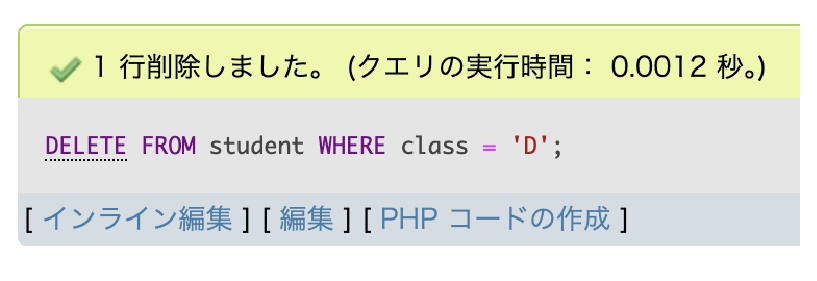
\includegraphics[width=80mm]{./fig/fig11.eps}
\caption{作製したコンデンサによる平滑回路を持つ全波整流回路の回路図}
\label{fig11}
\end{figure}

図\ref{fig11}に作製したコンデンサによる平滑回路を持つ全波整流回路を示す.

\begin{figure}[H]
\centering
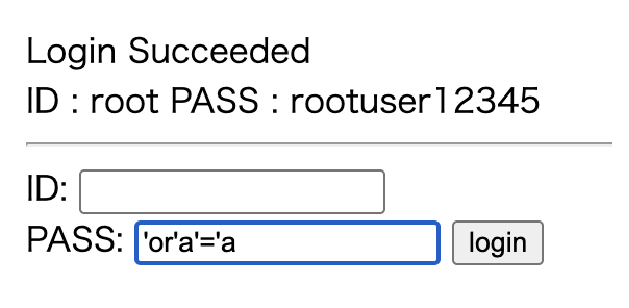
\includegraphics[width=80mm]{./fig/fig12.eps}
\caption{二次側の電圧と出力の波形}
\label{fig12}
\end{figure}

図\ref{fig12}に二次側の電圧$V_1$と出力$V_o$の波形を示す.

\subsubsection*{考察3}
ダイオードD1導通時,ダイオードD2導通時,ダイオード非導通時の時の電流の経路を示す.

\begin{itemize}
  \item ダイオードD1導通時\\
  変圧器の二次側からD1に流れ,$C$と$R_L$で分流した後,変圧器の2次側のセンタータップに流れる.
  \item ダイオードD2導通時\\
  変圧器の二次側からD2に流れ,$C$と$R_L$で分流した後,変圧器の2次側のセンタータップに流れる.
  \item ダイオード非導通時\\
  $C$の+から$R_L$に流れ,$C$の-に流れる.
\end{itemize}

\subsection{ツェナーダイオードの特性と基準電圧源}
整流回路の出力にコンデンサを挿入することで直流出力電圧の変動を小さくすることができた.
この実験では直流出力電圧をさらに抑えるための実験を行う.

\begin{figure}[H]
\centering
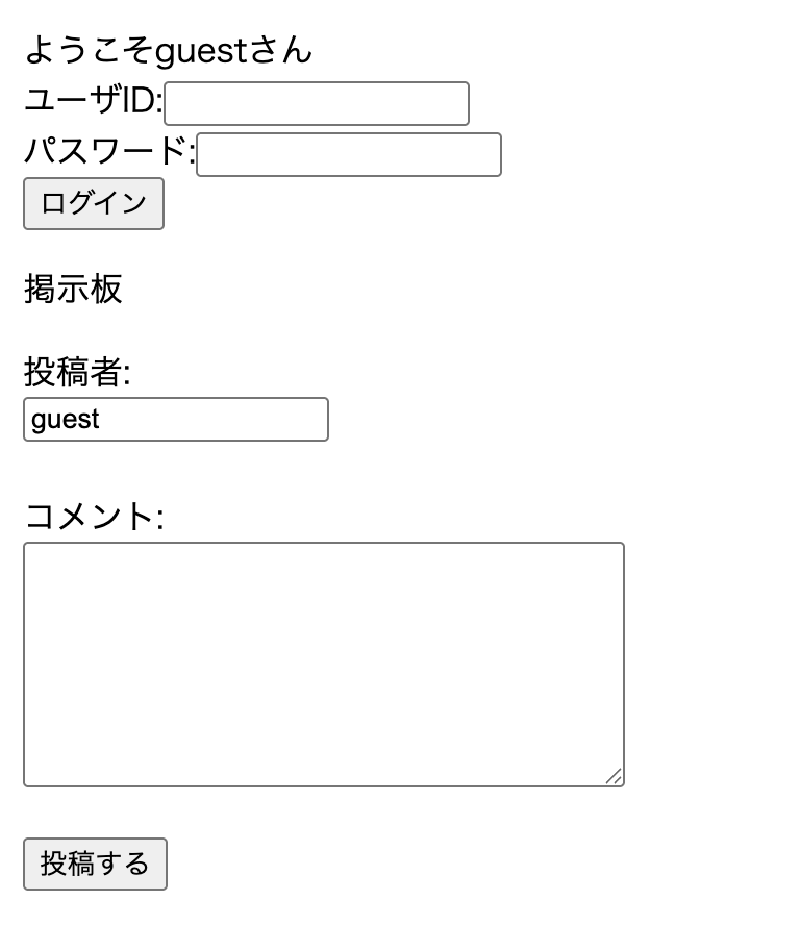
\includegraphics[width=80mm]{./fig/fig13.eps}
\caption{ツェナーダイオードを用いた基準電圧源の回路図}
\label{fig13}
\end{figure}

\subsubsection*{実験}
\begin{itemize}
  \item 図\ref{fig13}の回路を組み立てる.
  \item 電圧$V_1$の波形と出力$V_o$の波形をオシロスコープにより観測し,記録する.
\end{itemize}

\subsubsection*{結果}

\begin{figure}[H]
\centering
\includegraphics[width=80mm]{./fig/fig14.eps}
\caption{作製したツェナーダイオードを用いた基準電圧源の回路}
\label{fig14}
\end{figure}

図\ref{fig14}に作製したツェナーダイオードを用いた基準電圧源の回路を示す.

\begin{figure}[H]
\centering
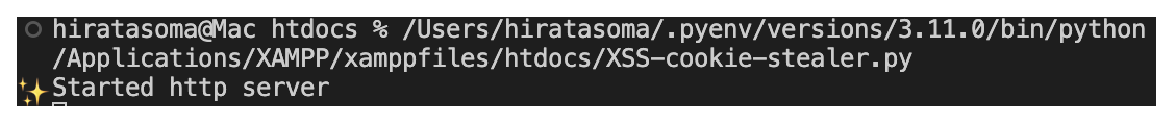
\includegraphics[width=80mm]{./fig/fig15.eps}
\caption{電圧$V_1$の波形と出力$V_o$の波形}
\label{fig15}
\end{figure}

図\ref{fig15}に観測した電圧$V_1$の波形と出力$V_o$の波形を示す.
\newpage

\subsubsection*{考察4}
オシロスコープの波形により,ツェナーダイオードに流れる電流$i$を求める.\\
図\ref{fig15}より,$V_o$は5.0V,$V_1$は9.8V〜7.0Vである.また抵抗$R$は510Ωなので,ツェナーダイオードに流れる電流$i$は,
\begin{gather}
i=\frac{V_1 - V_o}{R} \\
i_{max}=\frac{9.8 - 5.0}{510}=9.41[mA] \\
i_{min}=\frac{7.0 - 5.0}{510}=3.92[mA]
\end{gather}
となる.
よって,電流$i$は3.92mA〜9.41mAである.

\subsection{3端子レギュレータ特性}
トランジスタの特性を利用した3端子レギュレータの実験を行う.

\begin{figure}[H]
\centering
\includegraphics[width=80mm]{./fig/fig16.eps}
\caption{3端子レギュレータの回路図}
\label{fig16}
\end{figure}

\subsubsection*{実験}
\begin{itemize}
  \item 図\ref{fig16}の回路を組み立てる.
  \item $R_L=2[kΩ]$の時の電圧$V_i$の波形と出力$V_o$をオシロスコープにより観測し,記録する.
  \item $R_L=70[Ω]$の時の電圧$V_i$の波形と出力$V_o$をオシロスコープにより観測し,記録する.
\end{itemize}

\subsubsection*{結果}

\begin{figure}[H]
\centering
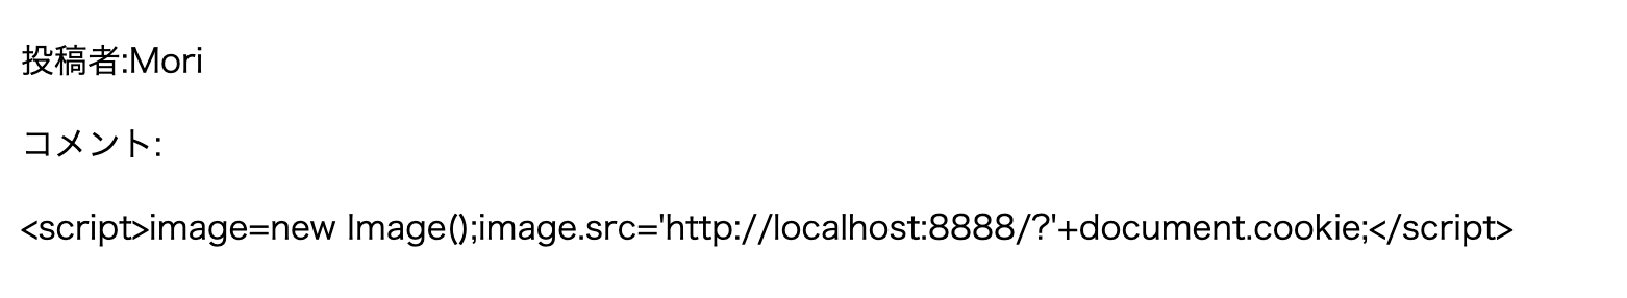
\includegraphics[width=80mm]{./fig/fig17.eps}
\caption{作製した3端子レギュレータ回路}
\label{fig17}
\end{figure}

図\ref{fig17}に作製した3端子レギュレータ回路を示す.

\begin{figure}[H]
\centering
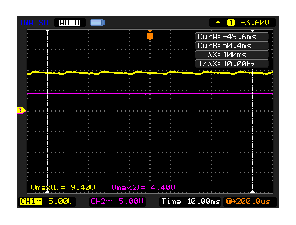
\includegraphics[width=80mm]{./fig/fig18.eps}
\caption{$R_L=2kΩ$の時の電圧$V_i$の波形と出力$V_o$の波形}
\label{fig18}
\end{figure}

\begin{figure}[H]
\centering
\includegraphics[width=80mm]{./fig/fig19.eps}
\caption{$R_L=70Ω$の時の電圧$V_i$の波形と出力$V_o$の波形}
\label{fig19}
\end{figure}

図\ref{fig18}と図\ref{fig19}にそれぞれ$R_L=2kΩ$の時と$R_L=70Ω$の時の電圧$V_i$の波形と出力$V_o$の波形を示す.

\subsubsection*{考察5}
3端子レギュレータの動作原理を説明する.\\
図\ref{fig16}に示した3端子レギュレータ回路はエミッタ接地回路と見ることができる.
よって,$V_o$はツェナーダイオードの電圧である5.1Vとトランジスタのベース・エミッタの電圧差である.
$V_1$が増加した場合,$R_1$の電圧が増加し,コレクタ・エミッタ電圧が増加する.
また,$V_1$が低下した場合,$R_1$の電圧が低下し,コレクタ・エミッタ電圧が低下する.
よって,$V_o$は一定に保たれる.

\subsection{出力可変型3端子レギュレータ}
図\ref{fig16}の回路により,直流出力電圧変動を抑えることができた.しかし,この回路では出力電圧はツェナーダイオードのツェナー電圧で固定されてしまう.
そこで,3端子レギュレータの直流電圧を可変とするような回路を作る.

\begin{figure}[H]
\centering
\includegraphics[width=80mm]{./fig/fig20.eps}
\caption{出力可変型3端子レギュレータの回路図}
\label{fig20}
\end{figure}

\subsubsection*{実験}
\begin{itemize}
  \item 図\ref{fig20}の回路を組み立てる.
  \item $VR_1$の$r$が$10kΩ$の時の$V_1, V_o, V_z, V_3$の波形をオシロスコープにより観測し記録する.
  \item $VR_1$の$r$が$50kΩ$の時の$V_1, V_o, V_z, V_3$の波形をオシロスコープにより観測し記録する.
  \item $VR_1$の$r$が$90kΩ$の時の$V_1, V_o, V_z, V_3$の波形をオシロスコープにより観測し記録する.
\end{itemize}

\begin{figure}[H]
\centering
\includegraphics[width=80mm]{./fig/fig21.eps}
\caption{作製した出力可変型3端子レギュレータ回路}
\label{fig21}
\end{figure}

図\ref{fig21}に作製した出力可変型3端子レギュレータ回路を示す.

\begin{figure}[H]
\centering
\includegraphics[width=80mm]{./fig/fig22.eps}
\caption{$VR_1$の$r$が$10kΩ$の時の$V_1, V_o$の波形}
\label{fig22}
\end{figure}

\begin{figure}[H]
\centering
\includegraphics[width=80mm]{./fig/fig23.eps}
\caption{$VR_1$の$r$が$10kΩ$の時の$V_z, V_3$の波形}
\label{fig23}
\end{figure}

\begin{figure}[H]
\centering
\includegraphics[width=80mm]{./fig/fig24.eps}
\caption{$VR_1$の$r$が$50kΩ$の時の$V_1, V_o$の波形}
\label{fig24}
\end{figure}

\begin{figure}[H]
\centering
\includegraphics[width=80mm]{./fig/fig25.eps}
\caption{$VR_1$の$r$が$50kΩ$の時の$V_z, V_3$の波形}
\label{fig25}
\end{figure}

\begin{figure}[H]
\centering
\includegraphics[width=80mm]{./fig/fig26.eps}
\caption{$VR_1$の$r$が$90kΩ$の時の$V_1, V_o$の波形}
\label{fig26}
\end{figure}

\begin{figure}[H]
\centering
\includegraphics[width=80mm]{./fig/fig27.eps}
\caption{$VR_1$の$r$が$90kΩ$の時の$V_z, V_3$の波形}
\label{fig27}
\end{figure}

\subsubsection*{考察6}
出力可変型3端子レギュレータの動作原理を説明する.\\
$V_o$が増加すると,Tr2 のベース電圧が増加し,コレクタ電圧が低下する.
そのため,$R_1$に流れる電流が増加し,$R_1$の電圧が増加する.すると,Tr1 のコレクタ・エミッタ電圧が
低下する.よって,$V_o$の電圧が減少し,一定に保たれる.
一方,$V_o$が減少すると,Tr2 のベース電圧が減少し,コレクタ電圧が増加する.そのため,
$R_1$に流れる電流が減少し,$R_1$の電圧が低下する.すると,Tr1 のコレクタ・エミッタ
電圧が増加する.よって,$V_o$の電圧が増加し,一定に保たれる。
$VR_1$を調節することで,Tr1 のベース電圧を変化し,Tr1 のコレクタ・エミッタ電圧が
変化する.そのため,$V_o$が変化する.

\subsection{三角波発生回路}

\begin{figure}[H]
\centering
\includegraphics[width=80mm]{./fig/fig28.eps}
\caption{三角波発生回路の回路図}
\label{fig28}
\end{figure}

三角波発生回路の周期T 理論値
\begin{gather}
T=\frac{4R_1R_3C}{R_2}
\end{gather}

\subsubsection{実験}
\begin{itemize}
  \item 図\ref{fig28}の回路を組み立てる.
  \item $V_2, V_3$の波形をオシロスコープにより観測し記録する.
\end{itemize}

\subsubsection{結果}
\begin{figure}[H]
\centering
\includegraphics[width=80mm]{./fig/fig29.eps}
\caption{作製した三角波発生回路}
\label{fig29}
\end{figure}

図\ref{fig29}に作製した三角波発生回路を示す.

\begin{figure}[H]
\centering
\includegraphics[width=80mm]{./fig/fig30.eps}
\caption{$V_2, V_3$の波形}
\label{fig30}
\end{figure}

図\ref{fig30}に$V_2, V_3$の波形を示す.

\subsubsection*{考察7}
波形より周期Tを求めて,理論値と比較する.\\
Tの理論値は$44.9μs$である.また,図\ref{fig30}より,Tの実測値は約$40.93μs$である.
よって,理論値と測定値の絶対誤差は$4.03μs$となった.これは,回路機器の誤差や配線の影響によるものであると考えられる.

\subsection{降圧チョッパ回路}
3端子レギュレータは効率の悪い電圧変動抑制法である.\\
効率の良い出力電圧抑制法であるチョッパ回路を学ぶ.

\begin{figure}[H]
\centering
\includegraphics[width=80mm]{./fig/fig31.eps}
\caption{降圧チョッパ回路の回路図}
\label{fig31}
\end{figure}

\subsubsection*{実験}
\begin{itemize}
  \item 図\ref{fig31}の回路を組み立てる.
  \item $V_o$の波形をオシロスコープにより観測し記録する.
\end{itemize}

\subsubsection*{結果}
\begin{figure}[H]
\centering
\includegraphics[width=80mm]{./fig/fig32.eps}
\caption{作製した降圧チョッパ回路}
\label{fig32}
\end{figure}

図\ref{fig33}に作製した降圧チョッパ回路を示す.

\subsubsection*{結果}
\begin{figure}[H]
\centering
\includegraphics[width=80mm]{./fig/fig33.eps}
\caption{降圧チョッパ回路の波形}
\label{fig33}
\end{figure}

図\ref{fig34}に降圧チョッパ回路の波形を示す.

\subsubsection*{考察8}
降圧チョッパ回路の特徴について述べる.

降圧チョッパ回路はスイッチング方式であるため,小型化でき,効率が良い.
しかし,トランジスタのスイッチングにより,ノイズが発生する.
また,コンデンサとインダクタによる過渡状態があり,瞬時に定常状態にならない.
\newpage

\subsection{降圧チョッパ回路のPWM制御法}
\begin{figure}[H]
\centering
\includegraphics[width=100mm]{./fig/fig34.eps}
\caption{降圧チョッパ回路のPWM制御方回路図}
\label{fig34}
\end{figure}

\subsubsection*{実験}
\begin{itemize}
  \item 図\ref{fig34}の回路を組み立てる.
  \item PWM制御回路の出力と$V_o$の波形を0オシロスコープにより観測し記録する.
\end{itemize}

\begin{figure}[H]
\centering
\includegraphics[width=150mm]{./fig/fig35.eps}
\caption{観測した降圧チョッパ回路のPWM制御回路の波形}
\label{fig35}
\end{figure}

図\ref{fig35}に観測した降圧チョッパ回路のPWM制御回路の波形を示す.

\begin{figure}[H]
\centering
\includegraphics[width=80mm]{./fig/fig36.eps}
\caption{作製した降圧チョッパ回路のPWM制御回路}
\label{fig36}
\end{figure}

図\ref{fig36}に作製した降圧チョッパ回路のPWM制御回路を示す.

\subsubsection*{考察9}
降圧チョッパ回路のPWM制御法の特徴について述べる.\\
PWMのデューティ比を大きくすると,$V_o$は$V_e$とほぼ等しくなる.
また,デューティ比を小さくすると,$V_o$は減少する.
しかし,過渡応答によって,$V_o$は瞬時に変化しない.

\subsection{昇圧チョッパ回路のPWM制御法}

\begin{figure}[H]
\centering
\includegraphics[width=100mm]{./fig/fig37.eps}
\caption{昇圧チョッパ回路のPWM制御方回路図}
\label{fig37}
\end{figure}

\subsubsection*{実験}
\begin{itemize}
  \item 図\ref{fig37}の回路を組み立てる.
  \item PWM制御回路の出力と$V_o$の波形をオシロスコープにより観測し記録する.
\end{itemize}

\subsubsection*{結果}
\begin{figure}[H]
\centering
\includegraphics[width=150mm]{./fig/fig38.eps}
\caption{観測した昇圧チョッパ回路のPWM制御回路の波形}
\label{fig38}
\end{figure}

図\ref{fig38}に観測した昇圧チョッパ回路のPWM制御回路の波形を示す.

\begin{figure}[H]
\centering
\includegraphics[width=80mm]{./fig/fig39.eps}
\caption{作製した昇圧チョッパ回路のPWM制御回路}
\label{fig39}
\end{figure}

図\ref{fig39}に作製した昇圧チョッパ回路のPWM制御回路を示す.

\subsubsection*{考察10}
昇圧チョッパ回路のPWM制御法の特徴について述べる.

PWMのデューティ比を大きくすると,$V_o$は増加する.
また,デューティ比を小さくすると,$V_o$は$V_e$に近づく.
しかし,過渡応答によって,$V_o$は瞬時に変化しない.

\subsubsection*{使用器具}
\begin{itemize}
  \item オシロスコープ:IWATSU DS-5105B
  S/N:BD174100219
  \item 2端子電源:TAKASAGO
  S/N:30290065
\end{itemize}

\newpage
\subsection*{感想}
電源回路には様々な種類があり,それぞれ特徴が異なることが分かった.
また,整流回路や平滑回路を用いることで,直流電圧を得ることができることが分かった.
さらに,3端子レギュレータやチョッパ回路を用いることで,効率的に電圧を制御できることが分かった.
今回の実験を通して,電源回路の基礎的な知識と実験技術を習得することができた.

\end{document}